% -*- coding: utf-8 -*-
\documentclass{article}
\usepackage[utf8]{inputenc}
\usepackage{CJKutf8}

\newenvironment{Korean}{%
 \CJKfamily{mj}}{}
\usepackage{graphicx}
\usepackage{caption}
\usepackage{mathtools}
\usepackage{listings, lstautogobble}
\usepackage{titlesec}
\usepackage{subcaption}
\usepackage{indentfirst}
\usepackage{makecell}

\begin{CJK}{UTF8}{}
\begin{Korean}

\title{ROS기반 GAZEBO 시뮬레이터 모바일 로봇 제작 및 구동 실험}
\author{박창규}
\date{2019년 3월 22일}
\titleformat{\paragraph}
{\normalfont\normalsize\bfseries}{\theparagraph}{1em}{}
\titlespacing*{\paragraph}
{0pt}{3.25ex plus 1ex minus .2ex}{1.5ex plus .2ex}

\begin{document}
	\maketitle
	\thispagestyle{empty}
	\newpage
	\paragraph{Abstract}
	로봇의 물성치와 구조를 정의한 urdf 파일을 사용하여 Gazebo 시뮬레이터 상에 모델을 제작하고, ROS를 이용하여 시뮬레이터 상의 로봇을 컨트롤하는 실험을 진행하였습니다. urdf 파일 작성시 xacro라는 ROS 패키지를 사용하여 반복되는 부분을 매크로화하였고, 로봇을 구성하고 있는 부분의 특성들은 특정한 재질을 가정하여 입력하였습니다. 작성한 urdf 파일은 rviz상에서 우선으로 구현하여 구조를 검증한 뒤, 시뮬레이터에 구현하였습니다. GAZEBO와 ROS의 실행은 launch 파일을 작성하여 진행하였고, 시뮬레이터의 ROS controller와 모델 생성 또한 launch 파일을 사용하여 진행하였습니다. 끝으로 구현된 로봇의 구동은 모델과 연결된 ROS controller node에 적절한 format의 rosmsg를 publish하여 진행하였습니다. 이 보고서는 앞에서 언급한 실험의 진행 과정과 의도한 부분의 검증 및 결론을 포함하고 있습니다.
	\tableofcontents
	\thispagestyle{empty}
	
	\newpage
	\setcounter{page}{1}
		
	\section{Introduction}
		\subsection{Robotics simulator}
		로보틱 시뮬레이터란 가상의 공간에 로봇을 3D 모델링과 렌더링으로 생성하고, 이와 대응하는 실제 로봇에 적용될 부분을 만들고 실험하는 소프트웨어입니다. 시뮬레이터가 되기 위해서는 실제 환경과 유사한 물리엔진, 다양한 물성치를 적용할 수 있는 부품과 가상 환경과 상호작용하는 센서 모델이 필요합니다. 시뮬레이터를 사용하면, 실제 로봇실험을 진행하는 것과 비교해 비용과 시간을 절약할 수 있습니다. 시뮬레이터에서 테스트한 어플리케이션은 연동 부분의 수정만으로 실제 로봇에 바로 적용하여 사용할 수 있습니다. 로보틱 시뮬레이터에는 Gazebo, Webots, Musoco 등 실험할 로봇의 목적에 따라 다양한 종류가 있습니다. 
		
		\subsection{Gazebo}
		Gazebo란 3차원 로봇 시뮬레이터 중 하나이고, OSRF(Open Source Robotics Foundation)에서 유지 관리를 하고 있습니다. 동사에서 제공하는 ROS와 연동하여 시뮬레이터 상에서 다양한 로봇 실험을 진행할 수 있습니다. 기본적으로 구현되어있는 모델 외에 ROS의 URDF 패키지를 사용하여 목적에 맞는 형태와 물성치를 가진 모델 및 센서를 생성할 수 있습니다.
		
		\subsection{ROS}
		ROS(Robot Operating System)는 로봇 시스템에 특화된 메타 운영체제로 하드웨어 추상화, 저수준 기기 제어 등 일반 운영체제에서 제공하는 기능들과 로봇 시스템을 위한 기능들이 함께 구현되어 있습니다. 이 실험에서는 Gazebo 시뮬레이터 상의 모델 생성과 생성된 모델의 제어에 사용하였습니다. 실험에 사용된 ROS 패키지와 도구의 대략적인 기능은 Table.\ref{table:rospackages}와 같습니다.
		
		\begin{table}[h]
		\centering
		\caption{ROS packages and tools used in experiment}
		\begin{tabular}{c|c}
			\textbf{Package \& Tool name} & \textbf{Usage}   \\
			\hline
			gazebo\_ros & 설정값을 적용한 Gazebo의 실행 및 urdf 모델의 생성\\
			\hline
			gazebo\_ros\_control & 로봇 컨트롤러 생성\\
			\hline
			controller\_manager & 로봇 컨트롤러 관리\\
			\hline
			xacro & 매크로를 활용한 urdf 모델 파일 제작\\
			\hline
			rviz & urdf 모델 시각화 및 검증\\
			\hline
			rqt\_graph & ROS node 관계도 시각화\\
		\end{tabular}
		\label{table:rospackages}
		\end{table}
		
	\section{Experiment}
		\subsection{Experimental system}
		\begin{figure*}[b!]
			\centering
			\begin{subfigure}[b]{0.5\textwidth}
			\centering
			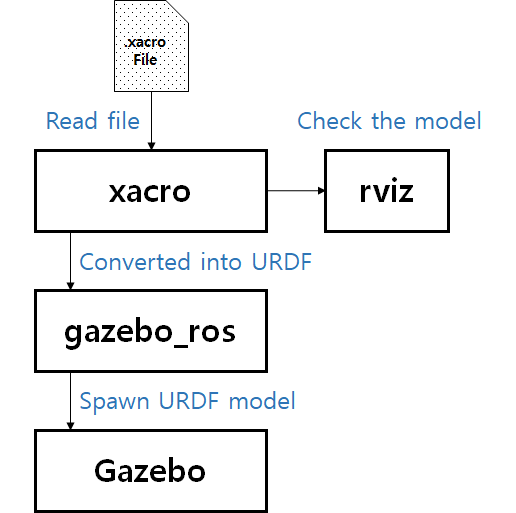
\includegraphics[width=\textwidth]{figures/spawn_model.png}
			\caption{\label{fig:spawn_model}Model spawn process}
			\end{subfigure}%
			~
			\begin{subfigure}[b]{0.5\textwidth}
			\centering
			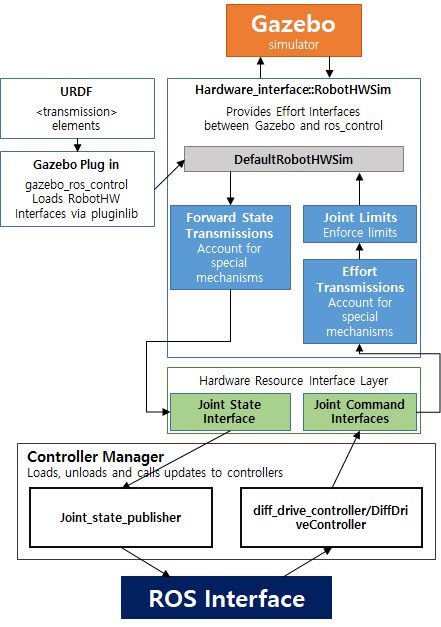
\includegraphics[width=\textwidth]{figures/control_system.png}
			\caption{\label{fig:control_system}Entire control system of experiment}
			\end{subfigure}
			\caption{About system}
		\end{figure*}
		
		전체 실험 시스템은 xacro 파일을 사용한 로봇 모델의 생성, 로봇을 작동하기 위한 조종부의 생성과 ROS 인터페이스를 이용한 조종으로 구성하였습니다.
		
			\subsubsection{Model spawning process}
			모델의 생성 과정은 Fig.\ref{fig:spawn_model}와 같습니다. 우선 xacro 포맷에 따라 모델 파일을 작성합니다. 작성된 파일에는 로봇의 물성치, 구조와 구동부에 대한 정보를 포함합니다. 그리고 모델을 Gazebo 상에서 생성하기 전에 rviz 기능을 통해 시각화하고 모델 파일을 잘 작성하였는지 검증합니다. 다음으로 xacro 패키지를 사용하여 .xacro 파일을 urdf 포맷으로 변환합니다. gazebo\_ros는 xacro 포맷도 지원하기 때문에 특정 명령어와 xacro 파일을 바로 사용하는 것도 가능합니다. 다음으로 gazebo\_ros 패키지를 사용하여 미리 실행된 Gazebo 시뮬레이터 상에 urdf 모델을 생성합니다.
			
			\subsubsection{Control system}
			Fig.\ref{fig:control_system}는 Control system의 구성을 도식화한 그림입니다. urdf의 transmission 부분을 따라 gazebo\_ros\_control 패키지를 사용해서 로봇의 가상 하드웨어 인터페이스를 생성합니다. 생성된 인터페이스에는 모델의 상태 정보를 제공하는 Forward State Transmissions와 모델의 구동을 제어하는 Effort Transmissions가 있습니다. ROS 인터페이스에서 입력되는 명령이나 인터페이스로 전송되는 데이터는 컨트롤러 매니저에서 관리하는 컨트롤러가 파싱하여 전달합니다. 로봇 보델과 컨트롤러 사이에는 둘 사이를 연결하는 Hardware Resource Interface Layer가 있습니다.

		\subsection{Model}
		모델 파일의 작성은 xacro 포맷으로 진행하였습니다. xacro란 urdf 파일에 매크로와 같은 몇가지 편의 기능들을 더한 패키지입니다. Gazebo 상에는 urdf 포맷으로 변환하여 적용됩니다. urdf는 크게 Link와 Joint로 구성되었습니다. Link에 적용되는 물성치는 특정한 물질을 가정하여 입력하였습니다.
		
			\subsubsection{Link}
			 Link에는 로봇의 각 부분의 형태 및 모양, 물리적 특성이 정의됩니다. 각 링크의 기능과 간단한 물성치는 Table.\ref{table:urdf_link}와 같습니다. base\_link와 left, right\_wheel의 색은 각각 하얀색과 파란색입니다.
			 		
			\begin{table}[h]
			\centering
			\caption{Information of urdf links}
			\begin{tabular}{c|c|c}
				\textbf{Link name} & \textbf{Function} & \textbf{Properties} \\
				\hline
				base\_link & 로봇의 중심 프레임 & \makecell{steel, density($kg/m^{3}$): 8050, \\ width(m): 0.3, length(m): 0.3, \\ height(m): 0.05,\\ coefficient of torsional friction: 1}\\
				\hline
				left\_wheel & 로봇의 왼쪽 바퀴 & \makecell{wood, density($kg/m^{3}$): 300, \\ width(m): 0.05, radius(m): 0.1, \\ coefficient of torsional friction: 1}\\
				\hline
				right\_wheel & 로봇의 오른쪽 바퀴 & same as left\_wheel\\
			\end{tabular}
			\label{table:urdf_link}
			\end{table}
			
			\subsubsection{Inertia moment and mass of link}
			Gazebo 상에서 실제와 같은 물성치를 부여하기 위해서는 형태에 맞는 관성 모멘트와 질량을 urdf 파일에 입력해주어야 합니다.
			우선 base\_link의 형태는 직육면체이므로 질량은 $mass=density*height*length*width$ 식을 통해 계산할 수 있습니다. 관성 모멘트의 값은 다음 식을 통해 얻을 수 있습니다.
			\begin{align}
			I_{xx} & =\frac{m*(a^2 + c^2)}{12} \\ 
			I_{yy} & =\frac{m*(b^2 + c^2)}{12} \\
			I_{zz} & =\frac{m*(a^2 + b^2)}{12} 
			\end{align}
			다음으로 각각의 wheel의 형태는 원통이므로 질량은 $mass=density*pi*radius^2*width$ 식을 통해 계산할 수 있습니다. 관성 모멘트의 값은 다음 식을 통해 얻을 수 있습니다.
			\begin{align}
			I_{xx} & = I_{yy} = \frac{m*(3r^2 + h^2)}{12} \\ 
			I_{zz} & =\frac{m*r^2}{2} 
			\end{align}
			
			
			\subsubsection{Joint}
			 Joint에는 링크와 링크사이의 연결을 정의할 수 있고, 자유도를 제한하여 힌지와 같은 연결부로 만들수 있습니다. 실험에서는 base\_link와 wheel을 연결하는 한 축의 회전 자유도를 갖는 한 종류의 Joint만 사용되었습니다. 해당 Joint의 상세 특성은 Table.\ref{table:urdf_joint}와 같습니다.
			 
			\begin{table}[h]
			\centering
			\caption{Properties of urdf joints}
			\begin{tabular}{c|l}
			\textbf{Joint name} & base\_to\_left,right\_wheel\_joint \\
			\hline
			\textbf{type} & continuous \\
			\hline
			\textbf{parent} & base\_link \\
			\hline
			\textbf{child} & left,right\_wheel\_joint \\
			\hline
			\textbf{degree of freedom} & 1(angular) \\
			\hline
			\textbf{damping} & 0\\
			\end{tabular}
			\label{table:urdf_joint}
			\end{table}
			
			\subsubsection{Visualization of model}
			\begin{figure*}[h]
				\centering
				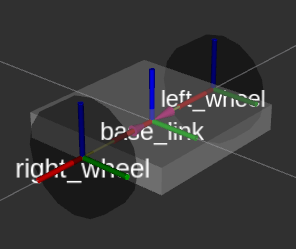
\includegraphics[width=0.3\textwidth]{figures/rviz_model.png}
				\caption{\label{fig:rviz_model}Visualization of model on rviz}
			\end{figure*}
			각각의 Link는 병렬이동과 축에 대한 회전을 통해 적절한 형태를 취하고 Joint를 통해 각각의 Link를 적절한 위치에 연결합니다. xacro 파일로부터 rviz를 통해 모델을 시각화하면 Fig.\ref{fig:rviz_model}와 같습니다. 시각화한 모델을 통해 잘 작성되었다는 것을 확인하였습니다.
			
			\subsubsection{Xacro file}
			모델의 urdf 파일 작성시 wheel 부분은 거울상으로 반전이 되지만 물성치 혹은 형태는 같습니다. 따라서 xacro 패키지를 통해 반복되는 부분을 간소화 해주는 macro 기능을 활용하여 파일의 내용을 간소화 하였습니다.

		\subsection{Model Controller}
		모델의 조작에 사용된 컨트롤러는 diff\_drive\_controller입니다. 모바일 로봇의 휠을 조작하는데 특화된 컨트롤러로써 velocity and acceleration limit과 같은 설정 값이 있습니다. 또한 정밀한 조작을 위해 모델의 특성을 입력해주어야 합니다. 우선 휠을 구동하는 Joint의 정보를 왼쪽과 오른쪽을 구분하여 설정해야하고, 바퀴 사이의 거리 역시 입력해주어야 합니다.
			
		\subsection{ROS packages}
			\subsubsection{Spawn model package}
			Gazebo를 실행하고 xacro 패키지를 사용한 모델과 Joint의 상태를 내보내는 컨트롤러를 생성하는 패키지입니다. 패키지 이름은 mobilerobot\_gazebo이고, 실행 방법은 다음과 같습니다.
			\begin{lstlisting}[autogobble=true, frame=single]
			$ cd ~/catkin_ws
			$ catkin_make
			$ source devel/setup.bash
			$ roslaunch mobilerobot_gazebo mobilerobot_urdf.launch
			\end{lstlisting}
			launch 파일을 통해 실행하며, 하위 디렉토리에 모델의 xacro file과 pid 설정 파일을 포함하고 있습니다.
			
			\subsubsection{Spawn controller package}
			생성된 모델의 구동부를 조작할 컨트롤러를 생성하는 패키지입니다. 패키지 이름은 mobilerobot\_control이고, 실행 방법은 다음과 같습니다.
			\begin{lstlisting}[autogobble=true, frame=single]
			$ cd ~/catkin_ws
			$ catkin_make
			$ source devel/setup.bash
			$ roslaunch mobilerobot_control mobilerobot_control.launch
			\end{lstlisting}
			또한 launch 파일을 통해 실행하며, 하위 디렉토리에 실험에서 사용된 diff\_drive\_controller의 설정 파일을 포함하고 있습니다.
			
			\subsubsection{Run the project}
			우선 패키지 폴더를 ROS의 작업 디렉토리 하위의 src 디렉토리로 옮깁니다. 이후에는 다음과 같이 명령어를 입력하면 실험을 실행할 수 있습니다.
			\begin{lstlisting}[autogobble=true, frame=single]
			$ cd ~/catkin_ws
			$ catkin_make
			$ source devel/setup.bash
			$ roslaunch mobilerobot_control mobilerobot_control.launch
			$ roslaunch mobilerobot_gazebo mobilerobot_urdf.launch
			$ rostopic pub /mobilerobot/mobilerobot_base_controller/\
			cmd_vel geometry_msgs/Twist -- \
			'[2.0, 0.0, 0.0]' '[0.0, 0.0, 1.8]'
			\end{lstlisting}
			로봇의 움직임은 Gazebo 상에서 렌더링되는 이미지를 통해 확인할 수 있습니다.
		
	\section{Result}
	\begin{figure*}[b!]
		\centering
		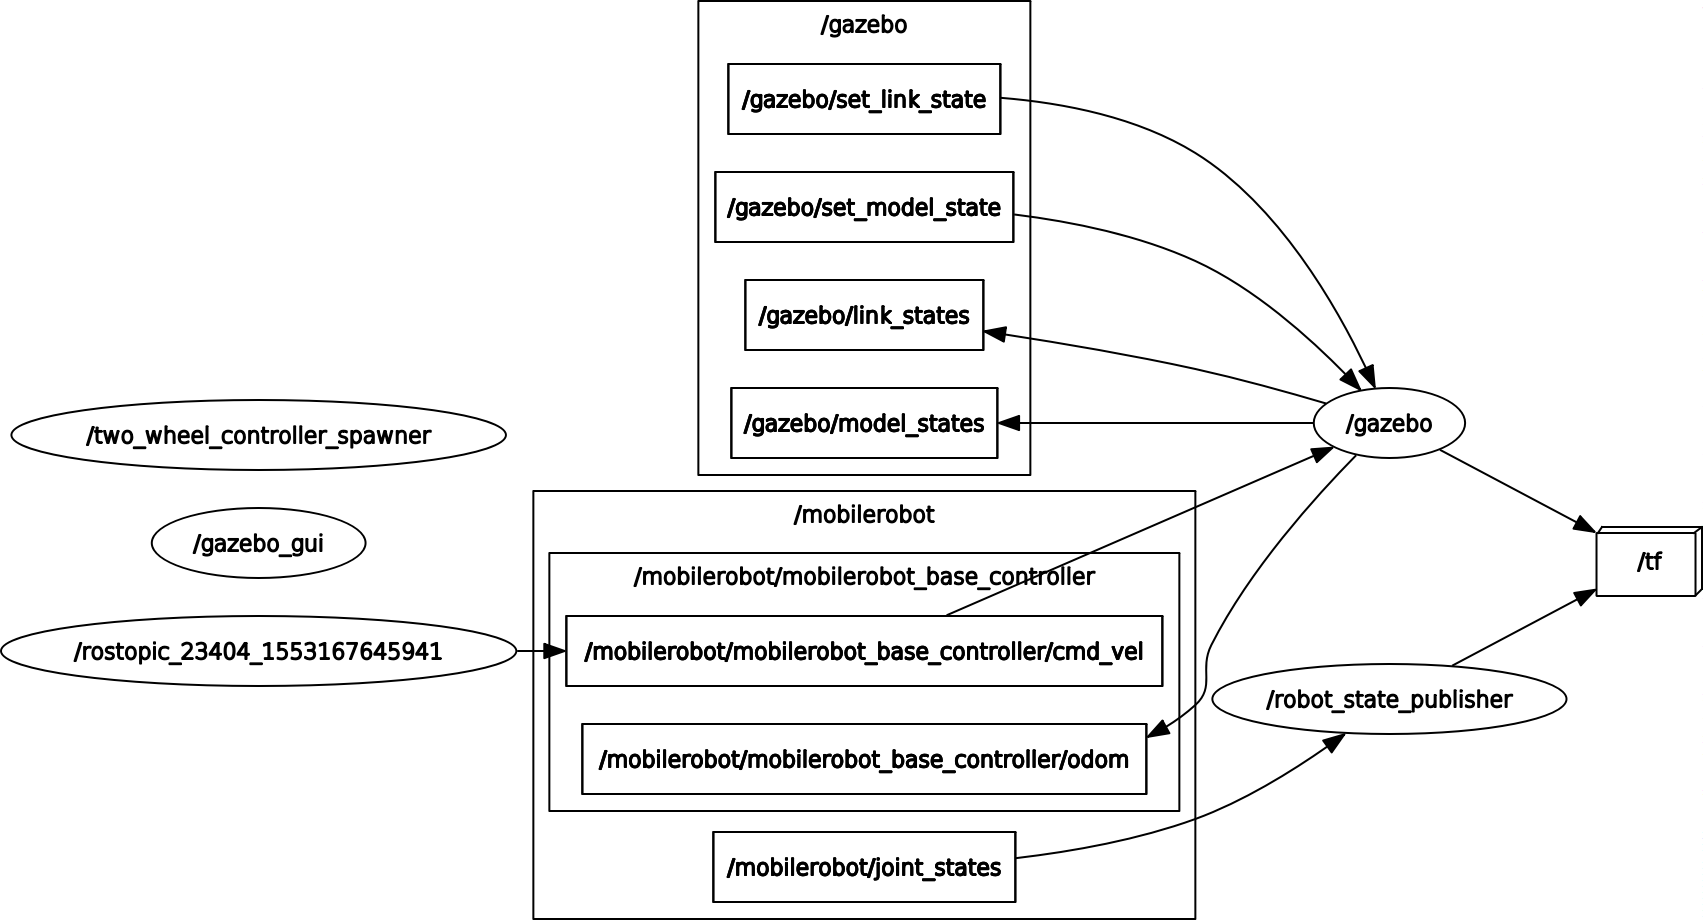
\includegraphics[width=0.95\textwidth]{figures/rqt_graph.png}
		\caption{\label{fig:rqt_graph}Visualization of nodes network}
	\end{figure*}
		
	\flushleft
	Fig.\ref{fig:rqt_graph}와 같이 rqt\_graph를 사용하여 생성된 ROS node들의 관계를 시각화하여 각 node 사이의 연결 상태를 확인하였습니다.\linebreak
	ROS 인터페이스인 rosmsg를 사용하여 모델에 작동 명령을 전달하여 모델이 동작하는 것을 확인하였습니다. 해당 실험 영상은 이 보고서와 함께 첨부되었습니다.\linebreak
	추가적으로 원통 형태의 기둥을 생성하고 로봇의 경로에 기둥을 배치하여 로봇의 진로를 방해 하였을때, 보이는 로봇의 반응을 확인하는 실험을 실시하였습니다. 추가 실험 영상 또한 첨부하였습니다.
	\section{Conclusion}
	실험을 실시한 결과 ROS node들 사이의 연결이 의도한대로 적절하게 구성되었다는 것을 확인하였습니다. 또한 시뮬레이터 상의 로봇의 동작을 확인한 결과 제공된 예제 동영상과 같이 실제 환경과 유사하게 작동한다는 것을 확인하였습니다.\linebreak
	실험을 통해 ROS 기반 Gazebo 시뮬레이터에서 물성치를 적용하여 모델과 구동부를 생성하는 방법과 ROS 인터페이스를 사용하여 Gazebo 상의 로봇에 명령을 전달하여 작동하고 시뮬레이션을 통해 데이터를 획득하는 과정을 실험을 통해 알게 되었고, 시뮬레이터를 이용하여 실제 환경에 적용하기에 앞서 가상의 실험을 통해 결과를 확인하고 가능성을 확인하는데 사용할 수 있습니다.\linebreak
	\indent 이번 실험에서는 로봇의 컨트롤과 시뮬레이터 상의 기본적인 정보만을 확인하였지만, 조사를 통해 여러가지 센서가 시뮬레이터에서 사용가능하다는 것을 확인하였습니다. 추가적으로 시뮬레이터에 몇가지 장애물을 추가하여 이번 실험과는 다른 가상 환경을 제작하고 센서를 부착하여 센서 데이터를 얻고 사용하는 추가적인 실험을 한다면 앞으로의 로봇 실험에 더 유용하게 사용할 수 있습니다.\linebreak
	\indent 또한 Asynchronous Reinforcement learning의 학습에서 현실의 실험과 현실과 비슷한 조건의 환경을 생성한 복수의 시뮬레이터를 병렬로 사용하여 가상환경의 실험을 동시에 진행하여 데이터를 취득한다면 학습 수렴 시간의 단축하는데도 적용할 수 있습니다.
	
\end{Korean}
\end{CJK}
\end{document}

